% -*- coding: utf-8; -*-

\chapter{Geração Semiautomática}
\label{gordon}

	Kindlmann e Durkin foram uns dos primeiros a gerar funções de transferência para visualizar as fronteiras de um volume de dados. Apesar de ter sido publicado há quase 20 anos e de possuir problemas na identificação de fronteiras em que a variação de seus valores se sobrepõem, seu trabalho ainda é o mais equilibrado no quesito \quote{Geração automática \textit{X} Controle do usuário}. Isso porque seu método gera bons resultados com uma função de transferência 1D exigindo uma intervenção mínima do usuário, ao mesmo tempo que o permite um controle fino sobre como a fronteira deve se apresentar visualmente.
	
	Neste Capítulo, o trabalho de \textit{Kindlmann e Durkin}~\cite{gordon} é apresentado em 4 seções. A seção~\ref{gordon.bound} define o conceito de fronteira e explica como identificá-las matematicamente. A geração da função de transferência 1D e 2D pode ser encontrada respectivamente nas seções~\ref{gordon.1d}~e~\ref{gordon.2d}. Por fim, o método é avaliado juntamente com alguns resultados, na seção~\ref{gordon.aval}.
	
	Afim de dinamizar a leitura desta dissertação, algumas simplificações serão utilizadas deste ponto em diante:
\begin{itemize}
	\item $s$ é um valor escalar qualquer contido no volume.
	\item Todas as funções que correspondem ao volume serão representadas por funções de uma única variável $x$.
	\item Todas as derivadas do volume são calculadas na direção do gradiente e portanto, representadas por $f'(x)$, $f''(x)$ e $f'''(x)$.
\end{itemize}
	
\section{Detecção de fronteiras}
\label{gordon.bound}
	\textit{Kindlmann e Durkin}~\cite{gordon} partem do princípio que toda fronteira é caracterizada por uma variação abrupta na intensidade de um material. Uma vez que também é assumido que os materiais são homogêneos, uma fronteira pode inicialmente ser modelada pela função degrau. No entanto, devido aos dispositivos responsáveis pela aquisição de dados, as fronteiras são comumente borradas com uma resposta gaussiana na frequência. Por esse motivo, o comportamento de uma fronteira em um volume de dados é melhor representado pela convolução da função degrau com uma gaussiana. O resultado dessa convolução é a função \textit{erf()}, ou função \textit{erro}, ilustrada na Figura~\ref{fig:boundary_model}.
	
\begin{figure}[h]
	\centering
	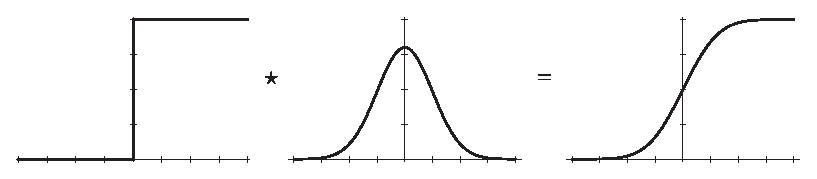
\includegraphics[width=1\textwidth]{images/g_boundary_model}
	\caption{Comportamento das funções degrau, gaussiana e erro, respectivamente~\cite{gordon}.}
	\label{fig:boundary_model}
\end{figure}

	A função \textit{erf()} é uma função contínua cuja imagem varia de $-1$ a $1$. Como uma fronteira pode variar entre quaisquer dois valores escalares contidos no volume, \textit{erf()} deve ser escalada para variar de $s_{min}$ a $s_{max}$. Assim, a função $f(x)$ que modela uma fronteira é definida pela equação~\eqref{eq:boundary} abaixo:

\begin{equation} \label{eq:boundary}
	f(x) = s = s_{min} + (s_{max} - s_{min}) \frac{1 + erf(\frac{x}{\sigma\sqrt{2}})}{2}
\end{equation}
	
	Por definição, a derivada direcional de uma função indica a taxa de variação dessa função em uma determinada direção...
	
	Apesar da fronteira poder variar entre $s_{min}$ e $s_{max}$, a Figura~\ref{fig:} mostra que a posição exata da fronteira encontra-se onde $f'(x)$ é máximo e $f''(x)$ é zero.
    
\section{Função de Transferência 1D}
\label{gordon.1d}
	Texto...
    
\section{Função de Transferência 2D}
\label{gordon.2d}    
    Texto..
    
\section{Avaliação do método}
\label{gordon.aval}    
    Atacar treshold do gordon, apresentando minha solução. Mas sem criticar de forma negativa.
    
    Comentar 2ª derivada média.
    
    Como bem ressaltado por \textit{Sereda et al.}~\cite{sereda1}, é comum esperar que aumentar a dimensão da função de transferência vá trazer melhores resultados e eliminar a sobreposição de fronteiras, mas frequentemente esse não é o caso. Por esse motivo, a intuitividade em assimilar e manipular uma FT 1D foi o que motivou
    
    
    Principalmente se analisado segundo a versão 1D de sua função de transferência. Seu método trás bons resultados sem exigir intervenção do usuário. E no caso da versão 1D a interface para ser gerada e ao mesmo tempo, a versão 1D é intuitiva
    
    
    Como visto no Capítulo~\ref{related}, o trabalho de \textit{Kindlmann e Durkin}~\cite{gordon} é o que menos exige iteração do usuário para detectar fronteiras automaticamente e, ao mesmo tempo, permitindo que este possa controlar a função de transferência gerada.
    Faça uma apresentação do método....extende o trabalho relacionado + introdução e (talvez) emende nesse início de deteção de fronteira...(talvez não rs).